% 5/22/2025 updated to use more common IEEEtran class file
% Bibliography commands are enabled because the included sections contain citations.
% see https://www.ieee.org/conferences/publishing/templates
\documentclass[11pt,final,conference]{IEEEtran}

\usepackage{physics,amsmath,amssymb,amsfonts}
\usepackage{algorithmic}
\usepackage{graphicx}
\usepackage{textcomp}
\usepackage{xcolor}
\usepackage{float}
\usepackage{booktabs}

%% wes 8/2021 additions
\usepackage{comment}    % wes 8/2021
\usepackage{color}      % wes 8/2021
\usepackage{listings}   % wes 8/2021

% wes: for code formatting/coloring
\definecolor{codegreen}{rgb}{0,0.6,0}
\definecolor{codegray}{rgb}{0.5,0.5,0.5}
\definecolor{codepurple}{rgb}{0.58,0,0.82}
\definecolor{backcolour}{rgb}{0.95,0.95,0.92}
\definecolor{codecyan}{rgb}{0.0,0.2,1.0}

% see: https://en.wikibooks.org/wiki/LaTeX/Source_Code_Listings
% set font, size, color style for code listings
\lstdefinestyle{mystyle}{
%    backgroundcolor=\color{backcolour},   
    commentstyle=\textcolor{codegreen},
%    keywordstyle=\color{magenta},    
    keywordstyle=\color{codecyan},
    numberstyle=\tiny\color{codegray},
    stringstyle=\color{codepurple},
    basicstyle=\ttfamily\footnotesize,
    breakatwhitespace=false,    
    breaklines=true,    
    captionpos=b,    
    keepspaces=true,    
    numbers=left,    
    numbersep=2pt,  
    firstnumber=auto,
    numberblanklines=false,
    showspaces=false,
    showstringspaces=false,
    showtabs=false,
    tabsize=2
}
% and then set mystyle to be the default when doing code listings
\lstset{style=mystyle}


\begin{document}

% these force page numbering to be turned on
\thispagestyle{plain}
\pagestyle{plain}


%% Paper title.

\title{Parallel MMUL \& LIKWID Performance Counters \\Assignment \#4, CSC 746, Fall 2026}

% IEEEtran way of specifying authors
\author{
\IEEEauthorblockN{Jacob Cordano}
\IEEEauthorblockA{Computer Science Department\\
San Francisco State University\\
San Francisco, CA, USA\\
Email: jcordano1@sfsu.edu}
}

\maketitle

%% Abstract section.
\begin{abstract}
Matrix multiplication is computationally expensive and sensitive to parallel scalability and memory locality. We implemented two matrix multiplication algorithms with OpenMP, one of which is a basic row parallel triple nested loop and another with cache blocking and thread local tile copies. Both algorithms were evaluated on the NERSC Perlmutter with block sizes of 128, 512, and 2048 using threads between 1 and 64, and measured with the Like I Know What I Knew What I'm Doing (LIKWID) API for runtime and cache utilization. At N = 2048, the basic and blocked implementations achieved 51x and 40x speedup at 64 threads, while the blocked implementation ran at 6x faster. The blocked algorithm also had significantly reduced L2 and L3 accesses relative to the basic implementation.
\end{abstract}

%% Abstract—Please take a few moments and try to compose an abstract for your homework writeup. It should contain these ideas: what was the problem being studied, what was the approach (what did you implement), what are the results. The abstract should describe the basic message of the paper, including: the problem, why your solution should be of interest, some notion that your solution is effective, and a teaser about how it has been evaluated. Cover all of this using between 75 and 150 words. Thus, the abstract is the hardest part to write. Sometimes I try to write it first, but the final version is usually composed of items drawn from the introduction, and then condensed, as the last step of writing the paper.

\section{Introduction}



\begin{comment}
%% the material that follows is from the generic tech paper skeleton project

The problem we have solved
\begin{itemize}
    \item Concentrate on making this assertion and only this assertion in a succinct set of 1 to 3 paragraphs
    \item A common mistake is to explain too much of the problem context first. Instead, state the problem essentially as a claim, and leave explanations supporting your claim to the next part, “Why it is not already solved.”
\end{itemize}

Why the problem is not already solved or other solutions are ineffective in one or more important ways
\begin{itemize}

\item Your new idea need not solve every problem but it should solve at least one that is not already solved
\item This is the place to provide a succinct description of the problem context giving enough information to support the claim that a problem exists, made in the preceding problem declaration.
  
\end{itemize}

Why our solution is worth considering and why is it effective in some way that others are not

\begin{itemize}
\item A succinct statement of why the reader should care enough to read the rest of the paper.
\item This should include a statement about the characteristics of your solution to the problem which 1) make it a solution, and 2) make it superior to other solutions to the same problem.
\end{itemize}

How the rest of the paper is structured
\begin{itemize}
    \item The short statement below is often all you need, but you should change it when your paper has a different structure, or when more information is required to describe what a given section contains. If it isn’t required then you don’t want to say it here.
\end{itemize}

The rest of this paper first discusses related work in Section 2, and then describes our implementation in Section 3. Section 4 describes how we evaluated our system and presents the results. Section 5 presents our conclusions and describes future work.

\end{comment}
% \input{02_relatedWork}

\section{Implementation}
\label{sec:implementation}
Here, we describe the implementation of the vector matrix multiplication algorithms (VMM) that we have developed and evaluated in this study. We first implement a basic matrix multiplication algorithm that has been parallelized using OpenMP. We then implement a blocked matrix multiplication algorithm that has also been parallelized using OpenMP. 

\subsection{DGEMM Basic Open MP Implementation}

The basic DGEMM implementation performs square matrix--matrix multiplication, computing \(C = C + AB\). The matrices are stored in row-major order. OpenMP parallelizes the outer loop over the rows of \(A\), allowing different threads to update distinct rows of \(C\) concurrently. For each output element \(C_{ij}\), the innermost loop computes the dot product of row \(i\) of \(A\) and column \(j\) of \(B\), adding the result to the existing value of \(C_{ij}\). Because each OpenMP iteration updates a distinct row of \(C\), no synchronization is required for the matrix updates. The LIKWID markers enclose the parallel computation for performance measurement.


\begin{lstlisting}[caption={Basic DGEMV OMP implementation}, label={lst:basic_dgemv}, name=dgemm_basic_omp, style=mystyle,language=C++]
void square_dgemm(int n, double *A, double *B, double *C){
    #pragma omp parallel
    {
        LIKWID_MARKER_START(MY_MARKER_REGION_NAME);

#pragma omp for
        for (int i = 0; i < n; i++)
        {
            for (int j = 0; j < n; j++)
            {
                double sum = C[i * n + j];
                for (int k = 0; k < n; k++)
                {
                    sum += A[i * n + k] * B[k * n + j];
                }
                C[i * n + j] = sum;
            }
        }

        LIKWID_MARKER_STOP(MY_MARKER_REGION_NAME);
    }
}
\end{lstlisting}

\subsection{DGEMM Blocked Open MP Implementation}

The blocked DGEMM computes \(C = C + AB\) for \(n \times n\) matrices \(A\), \(B\), and \(C\), all stored in row-major order. The matrices are divided into square tiles with dimensions \texttt{block\_size} by \texttt{block\_size}. Each tile of \(C\) is copied into a thread-local buffer and updated using the corresponding tiles of \(A\) and \(B\), which are also copied into thread-local buffers. This copy optimization improves spatial and temporal locality by allowing the block multiplication to operate on contiguous data that can be reused from the cache. OpenMP parallelizes the outer loop over block rows, allowing threads to update distinct regions of \(C\) concurrently without requiring synchronization. After all contributing block products have been accumulated, the updated tile is copied back into \(C\). The LIKWID markers enclose the parallel computation for performance measurement. 

\begin{lstlisting}[caption={Blocked DGEMV OMP pseudocode implementation}, label={lst:blocked_dgemv}, name=dgemm_blocked_omp, style=mystyle,language=C++]
PROCEDURE Blocked_DGEMM(n, size, A, B, C)
    blocks = n / size

    PARALLEL FOR each block (i, j)
        Copy C(i,j) to local C_block

        FOR k = 0 TO blocks - 1
            Copy A(i,k) to local A_block
            Copy B(k,j) to local B_block
            C_block = C_block + A_block * B_block
        END FOR

        Copy C_block back to C(i,j)
    END PARALLEL FOR
END PROCEDURE
\end{lstlisting}

\section{Results}

\subsection{Computational platform and Software Environment}

This evaluation was performed on the NERSC Perlmutter supercomputer using two AMD EPYC 7763 processors with a base clock speed of 2.45~GHz. The system was configured with 512~GB of DDR4 memory per node, a 32~KB L1 cache, a 512~KB L2 cache, and a 32~MB L3 cache, providing ample resources for large matrix multiplications. The operating system is SUSE Linux Enterprise Server 15~SP6 with kernel version \texttt{6.4.0\char45 150600.23.125\_15.0.29\char45 cray}\\ \texttt{\detokenize{_shasta_c}}. GCC 14.3.0 and CMake 3.28.3 were used for compilation and build configuration, respectively. \cite{nersc}

\subsection{Methodology}

While conducting this evaluation, we focused on measuring the performance of our matrix multiplication implementations under various configurations. We utilized OpenMP for parallelization and compared the performance of our Basic Matrix Multiplication, Blocked Matrix Multiplication, and the CBLAS library. The evaluation was conducted across different problem sizes, specifically 128, 512, and 2048, to assess scalability and efficiency. We collected data on execution time, speedup, and cache access patterns to provide a comprehensive understanding of the performance characteristics of each implementation.

All metrics were collected using the job files which leveraged the LIKWID performance monitoring tool, allowing us to capture detailed information about speedup using the Runtime (RDTSC) values as well as cache access patterns using the L2 and L3 cache access counters. The collected data was then analyzed to identify trends, bottlenecks, and areas for optimization.

\subsection{Scaling Study for Basic MM with OpenMP parallelization}

The scaling study for basic matrix multiplication with OpenMP parallelization was conducted to evaluate the performance improvements achieved through parallel execution. The study involved running the Basic MM implementation across different problem sizes and measuring the speedup achieved by utilizing multiple threads.

To collect this data, we executed the included job-basic-omp file, which was designed to run the Basic MM implementation with OpenMP parallelization. The job file was configured to utilize multiple threads, allowing us to observe the performance gains achieved through parallel execution.

The problem sizes tested were 128, 512, and 2048, and the speedup was calculated by comparing the execution time of the parallel implementation against the serial version. The results of this scaling study are presented in Figure~\ref{fig:basic_openmp_comparison}, which illustrates the speedup achieved for each problem size.

Speedup was calculated using the formula:
\begin{equation}
    \text{Speedup} = \frac{\text{Execution Time (Serial)}}{\text{Execution Time (Parallel)}}
\end{equation}

The execution time for the parallel implementation was measured using the maximum runtime recorded across all threads, while the serial execution time was obtained from the single-threaded execution of the Basic MM implementation. The reason for using the maximum runtime across threads is to account for the fact that the overall execution time is determined by the slowest thread, which can be influenced by factors such as load imbalance and thread synchronization overhead.

Figure~\ref{fig:basic_openmp_comparison} shows the speedup by problem size for the basic matrix multiplication implementation parallelized with OpenMP.

\begin{figure}[H]
    \centering
    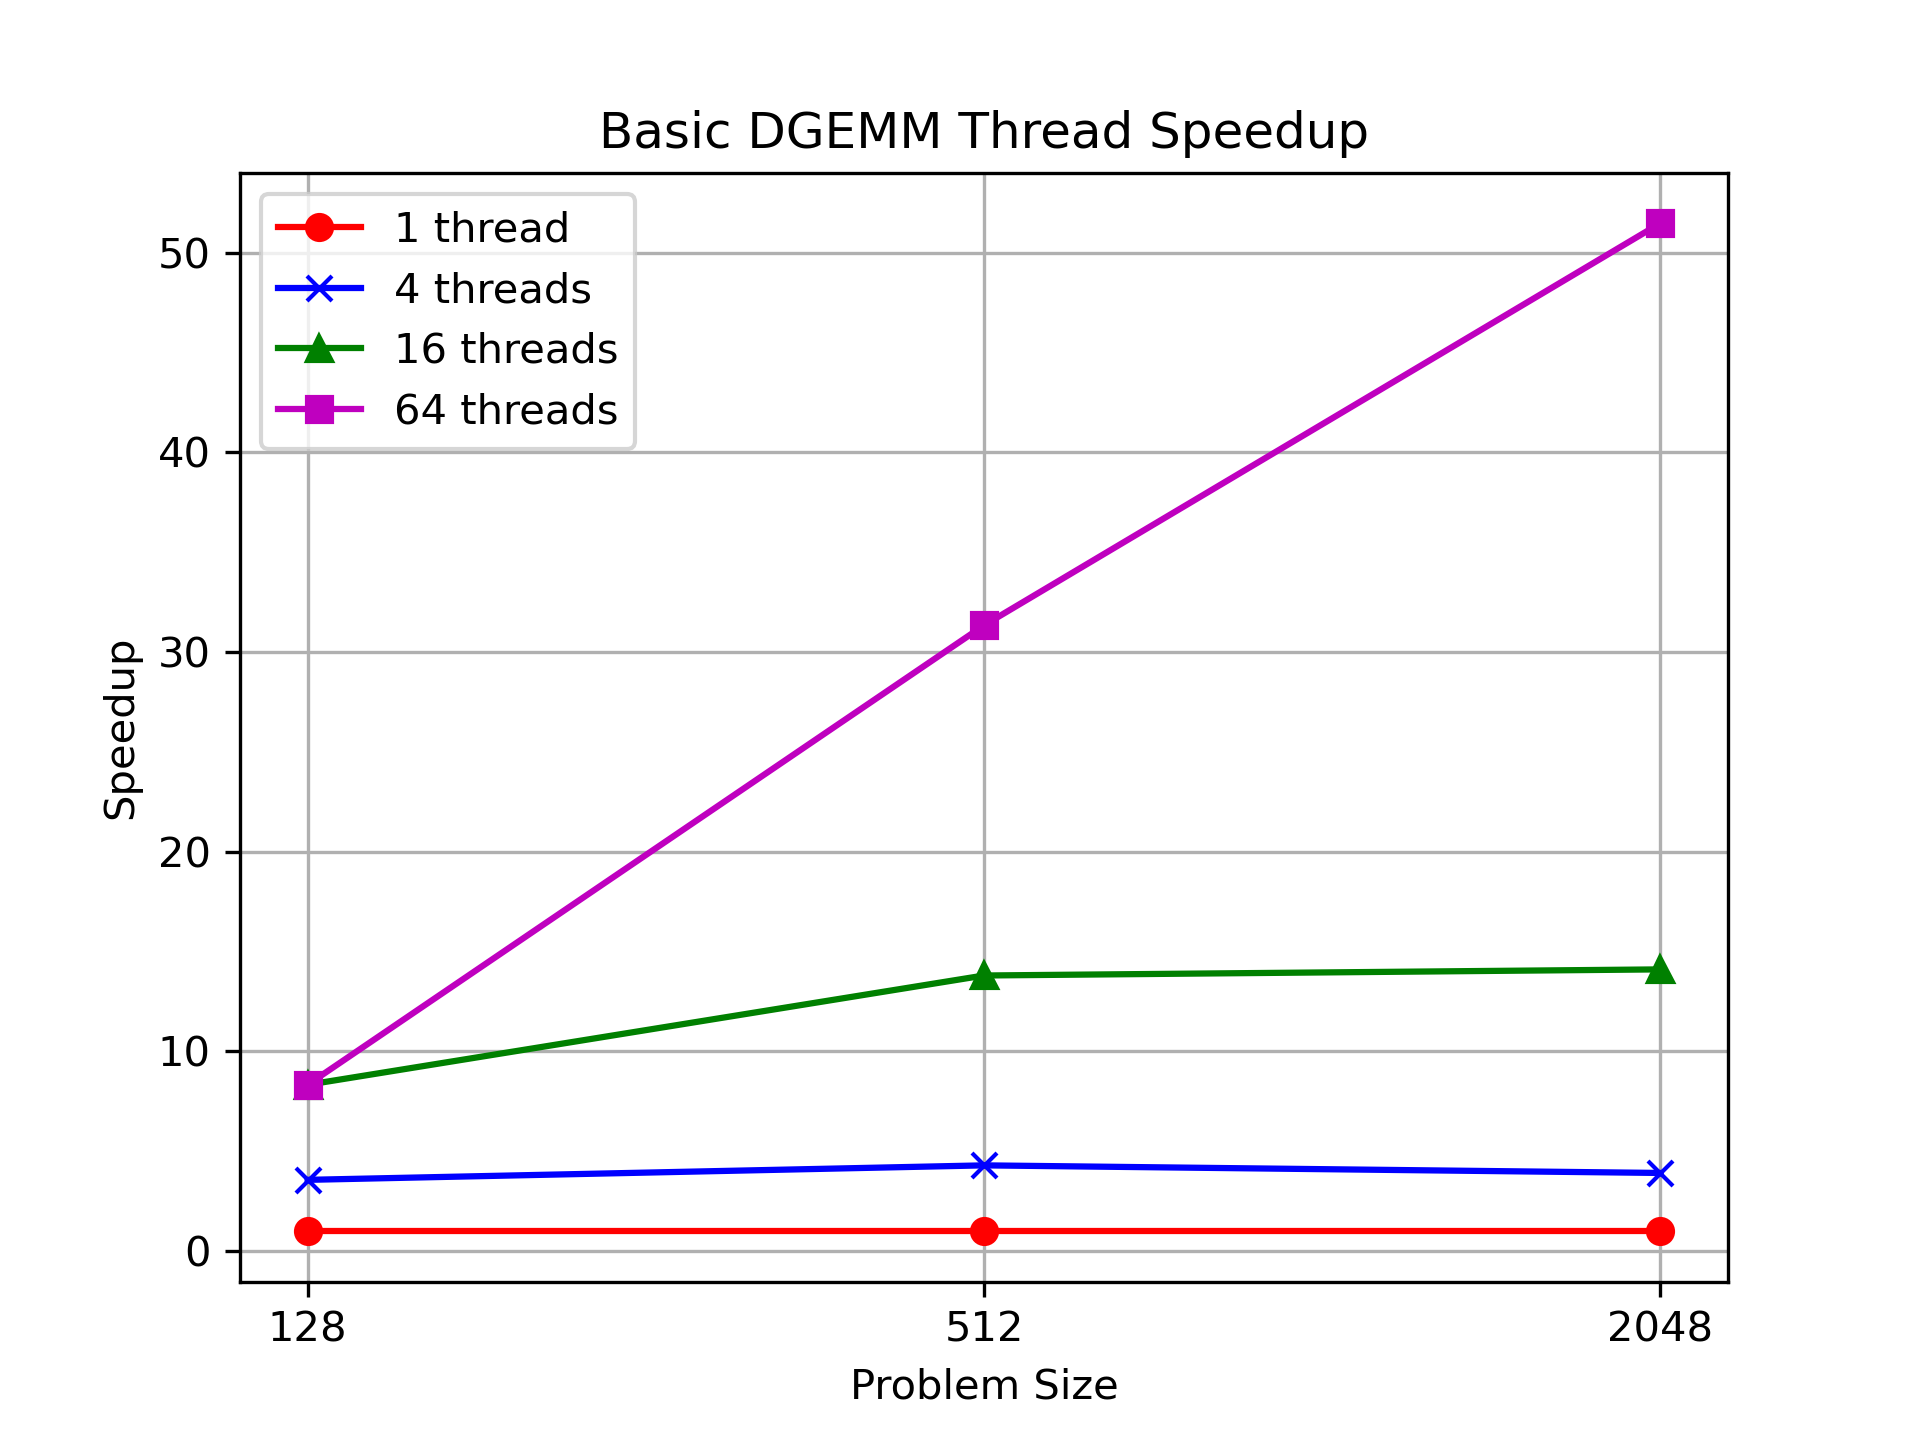
\includegraphics[width=.75\linewidth]{images/basic_speedup.png}
    \caption{Speedup of Basic Matrix Multiplication with OpenMP parallelization}
    \label{fig:basic_openmp_comparison}
\end{figure}

We observed that the speedup achieved by the Basic implementation was significant as concurrency increased, with the highest speedup observed for the largest problem size of 2048 and a concurrency of 64 threads. We also observed that speedup was not linear as well and see that problem size seems to have the most significant increases on the 64-thread speedup. This is likely due to the greater ability to utilize the available threads for larger problem sizes.

\subsection{Evaluation of BMMCO with OpenMP parallelization}

For the blocked matrix multiplication implementation with OpenMP parallelization, we conducted a similar scaling study to evaluate its performance improvements. The study involved running the blocked implementation across different problem sizes and measuring the speedup achieved by utilizing multiple threads.

To collect this data, we executed the included job-blocked-omp file, which was designed to run the blocked implementation with OpenMP parallelization. The job file was configured to utilize multiple threads, allowing us to observe the performance gains achieved through parallel execution.

To calculate speedup, we used the same formula as in the previous section, comparing the execution time of the parallel implementation against the serial version. The execution time for the parallel implementation was measured using the maximum runtime recorded across all threads, while the serial execution time was obtained from the single-threaded execution of the blocked implementation.

Figure~\ref{fig:blocked_openmp_comparison} shows the speedup by problem size for the blocked implementation parallelized with OpenMP. 

 \begin{figure}[H]
    \centering
    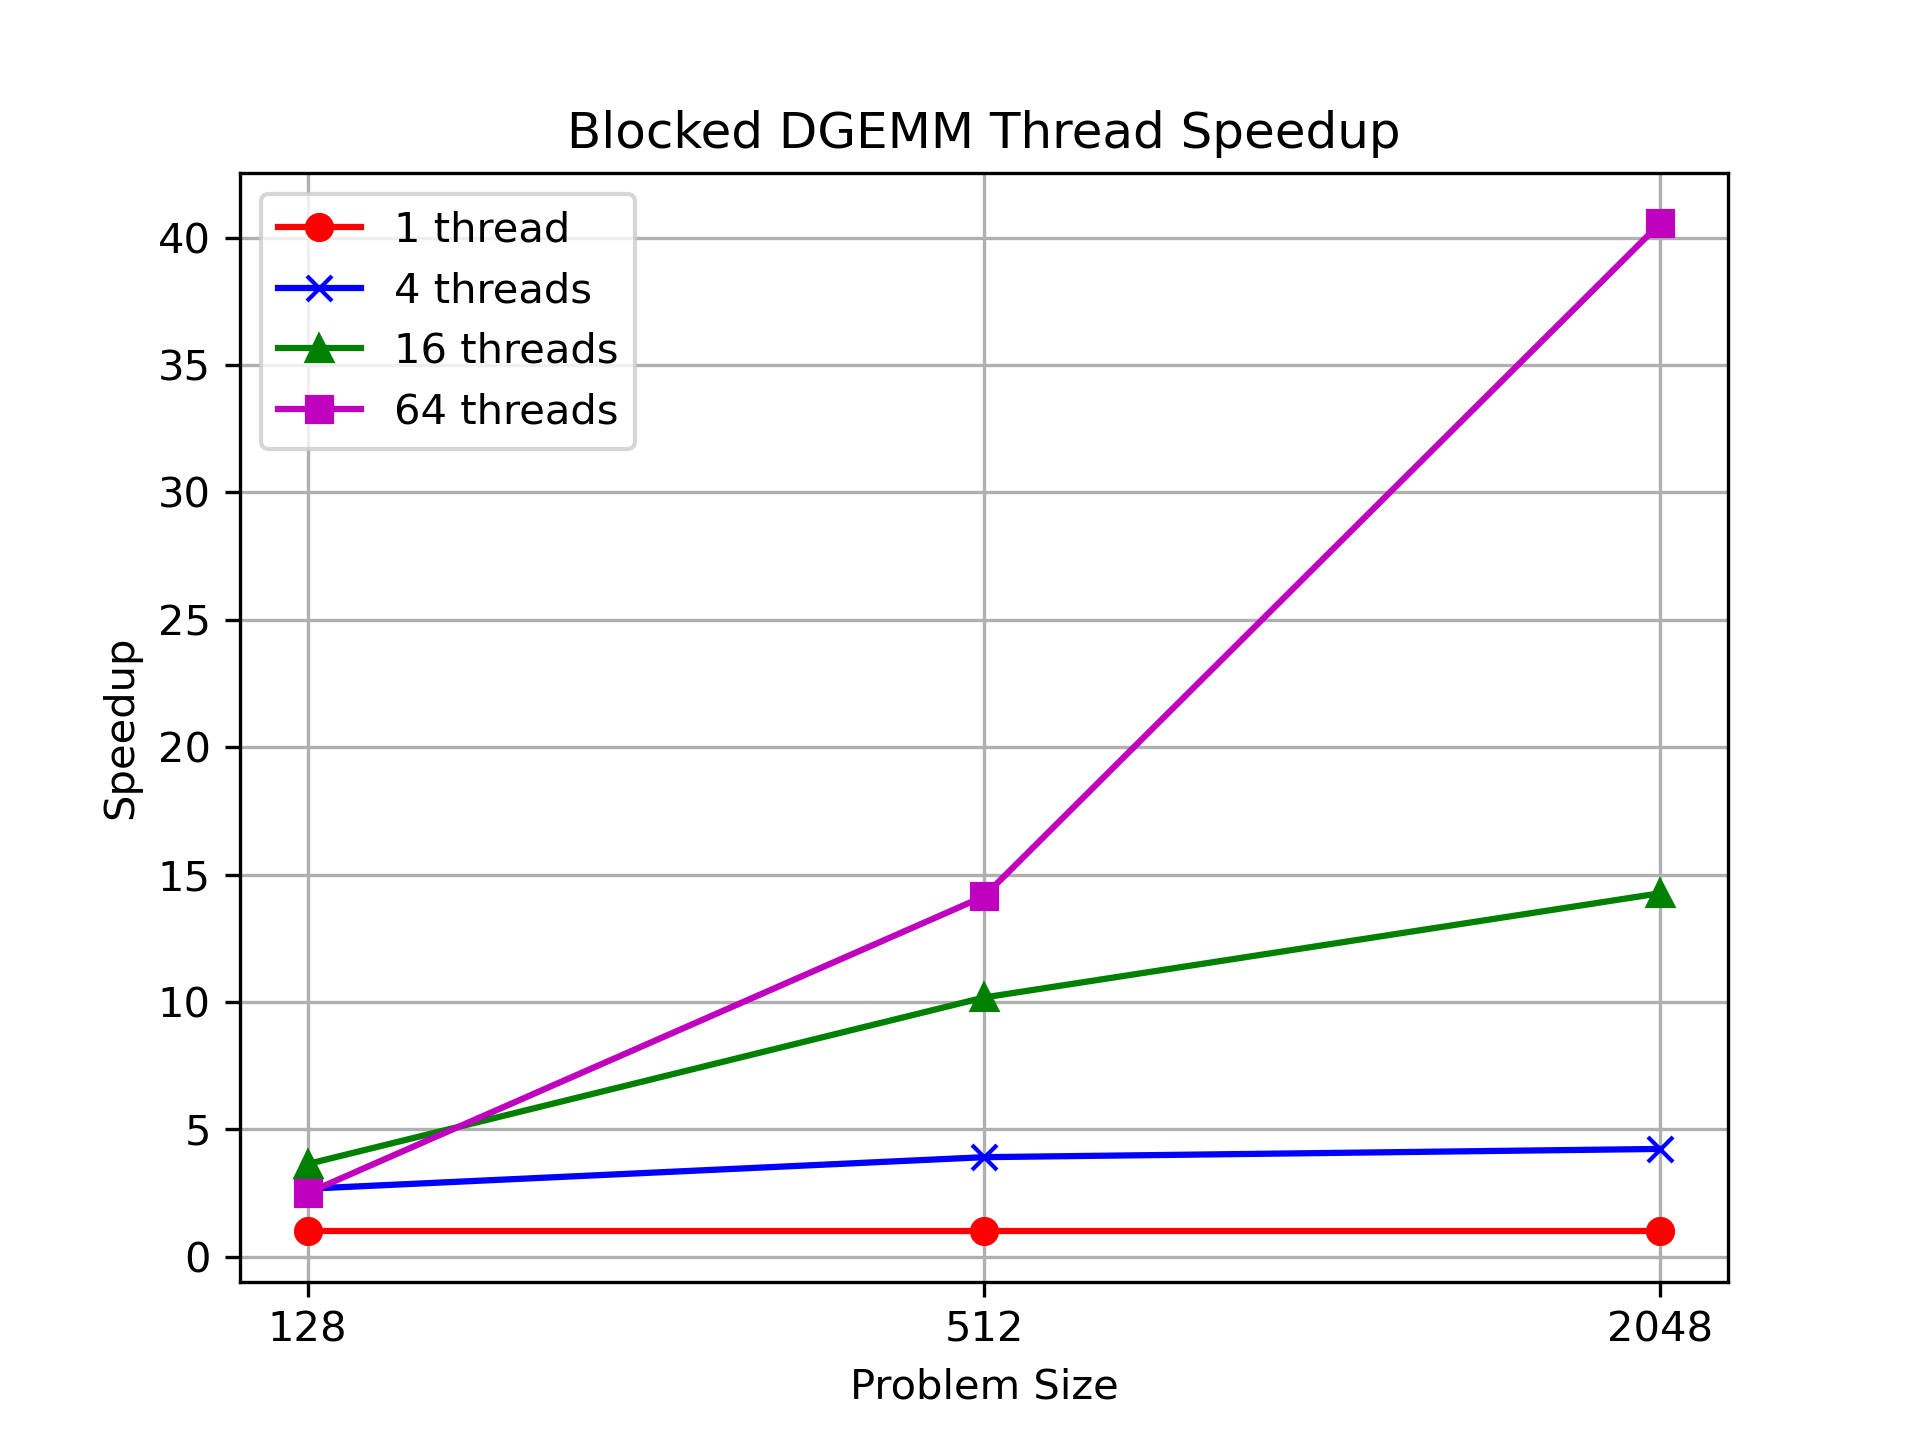
\includegraphics[width=.75\linewidth]{images/blocked_speedup.png}
    \caption{Speedup of Blocked Matrix Multiplication with OpenMP parallelization}
    \label{fig:blocked_openmp_comparison}
\end{figure}

In this observation, we found that speedup was less significant for the blocked implementation compared to the basic implementation. The highest speedup was observed for the largest problem size of 2048 and a concurrency of 64 threads, but the overall speedup was lower than that of the basic implementation. Additionally, we observed that the different problem sizes had generated elevated speedup for the threads less than 64 when compared tot the basic implementation.

The lower overall speedup for the blocked implementation can be attributed to the increased complexity of the algorithm compared to the basic implementation, which may introduce additional computational overhead.

\subsection{Comparison of CBLAS, BasicMM-omp, and BMMCO-omp}

\begin{table}[H]
    \centering
    \caption{Normalized L2 cache accesses. Each value is divided by the
    corresponding CBLAS L2 access count for the same problem size.}
    \label{tab:normalized_l2_accesses}
    \small
    \begin{tabular}{@{}rcccc@{}}
        \toprule
        Problem size & CBLAS & Basic & Blocked B4 & Blocked B16 \\
        \midrule
        128  & 1.000 & 44.987  & 4.574  & 1.335 \\
        512  & 1.000 & 45.813  & 4.449  & 1.977 \\
        2048 & 1.000 & 120.906 & 7.807  & 2.013 \\
        \bottomrule
    \end{tabular}
\end{table}

\begin{table}[H]
    \centering
    \caption{Normalized L3 cache accesses. Each value is divided by the
    corresponding CBLAS \texttt{L3\_ACCESS\_ALL\_TYPES} count for the same
    problem size.}
    \label{tab:normalized_l3_accesses}
    \small
    \begin{tabular}{@{}rcccc@{}}
        \toprule
        Problem size & CBLAS & Basic & Blocked B4 & Blocked B16 \\
        \midrule
        128  & 1.000 & 0.044   & 0.035  & 0.053 \\
        512  & 1.000 & 273.351 & 13.936 & 3.043 \\
        2048 & 1.000 & 604.116 & 20.994 & 4.508 \\
        \bottomrule
    \end{tabular}
\end{table}


\subsection{Overall findings and discussion}


\section{AI Usage}

In order to complete this assignment AI was used in the following ways:

\begin{itemize}
    \item To configure the included Dockerfile so that I may easily run the homework file without installing various packages locally to my machine.
    \item After running the benchmarks, I would ask an LLM to combine data into one CSV for plotting.
    \item For LaTeX debugging, formatting, and learning how to use citations.
    \item To create my speedup LaTeXtable.
    \item To better understand the lecture materials provided for the course.
\end{itemize}


%\bibliographystyle{abbrv}
\bibliographystyle{abbrv-doi}
%\bibliographystyle{abbrv-doi-narrow}
%\bibliographystyle{abbrv-doi-hyperref}
%\bibliographystyle{abbrv-doi-hyperref-narrow}

% Include the current references until they are cited explicitly in the text.
\nocite{*}
\bibliography{template}
\end{document}
